%\addtocontents{toc}{\setlength\cftchapternumwidth{1em}}
%\renewcommand\thechapter{}


\chapter{Trigger scale factors}
%\renewcommand{\thechapter}{A}
\label{app:TriggerSF}



The trigger scale factors measured as a function of lepton \pt, using the dataset collected by \Etmis\ triggers and \WZ\ simulation, after a 3 lepton and jets selection, in the Z mass window. All corrections to simulation are applied.



\begin{table}[htbp]
	\centering
	\caption{Trigger efficiencies on data events selected with \Etmis\ triggers and \WZ\ simulation for all leptonic channels together. The unweighed number of events is quoted. When there are no events passing the cuts, it is indicated with N/A. The uncertainties are statistical uncertainties.}
	\begin{tabular}{c|c|c|c|c}
		\toprule
		ALL CHANNEL & \multicolumn{2}{c|}{data} & \multicolumn{2}{c}{WZ simulations} \\ 
		& Efficiency & unc. & Efficiency & unc. \\
		\midrule 
		3 lep,  at least one jet & 117/118 = 99.15 \% & 12.94\% & 18047/18055 = 99.96\%  & 1.05\% \\ 
		\hline 
		\STSR & 6/6 = 100.00\% & 57.74\% & 1541/1541 = 100.00\% & 3.60\% \\ 
		\hline 
		\TTSR & 26/27 = 96.30\% & 26.46\% & 1791/1792 = 99.94\% & 3.34\% \\ 
		\hline 
		\WZCR & 69/69 = 100.00 \% & 17.03\% & 14405/14412=99.95\% & 1.18\% \\ 
		\bottomrule 
	\end{tabular} 
\end{table}	
\begin{table}[htbp]
	\centering
	\caption{Trigger efficiencies on data events selected with \Etmis\ triggers and \WZ\ simulation for \mumumu\ leptonic channel together. The unweighed number of events is quoted. When there are no events passing the cuts, it is indicated with N/A. The uncertainties are statistical uncertainties.}
	\begin{tabular}{c|c|c|c|c}
		\toprule 
		\mumumu\ CHANNEL & \multicolumn{2}{c|}{data} & \multicolumn{2}{c}{\WZ\ simulations} \\
		& Efficiency & unc. & Efficiency & unc. \\ 
		\midrule 
		3 lep,  at least one jet & 40/40 = 100.00 \% & 22.36 \% & 7814/7814 = 100.00\%  & 1.60\% \\ 
		\hline 
		\STSR & N/A & N/A & 687/687 = 100\% & 5.40\% \\ 
		\hline 
		\TTSR & 13/13 = 100.00\% & 39.22\% &763/763 = 100.00\% & 5.12\% \\ 
		\hline 
		\WZCR & 22/22 = 100.00 \% & 30.15\% & 6238/6238=100.00\% & 1.79\% \\ 
		\bottomrule
	\end{tabular} 
\end{table}	
\begin{table}[htbp]
	\centering
	\caption{Trigger efficiencies on data events selected with \Etmis\ triggers and \WZ\ simulation for \eee\ leptonic channel together. The unweighed number of events is quoted. When there are no events passing the cuts, it is indicated with N/A. The uncertainties are statistical uncertainties.}

	\begin{tabular}{c|c|c|c|c}
		\toprule 
		\eee\ CHANNEL & \multicolumn{2}{c|}{data} & \multicolumn{2}{c}{WZ simulations} \\ 
		& Efficiency & unc. & Efficiency & unc. \\
		\midrule
		3 lep,  at least one jet & 20/21 = 95.24\%  & 29.76\% & 2211/2215 = 99.82 \% & 3.00\%  \\ 
		\hline 
		\STSR & 4/4 = 100.00\% & 70.71\% & 176/176 = 100.00\% & 10.66\% \\ 
		\hline 
		\TTSR & 2/3 = 66.67\% & 60.86\% & 242/242 = 100.00\% & 9.09\% \\ 
		\hline 
		\WZCR & 14/14 = 100.00 \% & 37.80\% & 1744/1748=99.77\% & 3.38\% \\ 
		\bottomrule
	\end{tabular} 
\end{table}
\begin{table}[htbp]
	\centering
	\caption{Trigger efficiencies on data events selected with \Etmis\ triggers and \WZ\ simulation for \eemu\ leptonic channel together. The unweighed number of events is quoted. When there are no events passing the cuts, it is indicated with N/A. The uncertainties are statistical uncertainties.}

	\begin{tabular}{c|c|c|c|c}
		\toprule
		\eemu\ CHANNEL & \multicolumn{2}{c|}{data} & \multicolumn{2}{c}{WZ simulations} \\ 
		& Efficiency & unc. & Efficiency & unc. \\
		\midrule
		3 lep,  at least one jet & 32/32 = 100.00 \% & 25.00 \% & 3116/3118 = 99.94\%  & 2.53\% \\ 
		\hline 
		\STSR & 1/1 = 100.00\%& 141.42\% & 255/255 = 100\% & 8.86\% \\ 
		\hline 
		\TTSR & 9/9 = 100.00\% & 47.14\% &291/291 = 100.00\% & 8.29\% \\ 
		\hline 
		\WZCR & 14/14 = 100.00 \% & 37.80\% & 2529/2531=99.92\% & 2.81\% \\ 
		\bottomrule
	\end{tabular} 
\end{table}	
\begin{table}[htbp]
	\centering
	\caption{Trigger efficiencies on data events selected with \Etmis\ triggers and \WZ\ simulation for \emumu\ leptonic channel together. The unweighed number of events is quoted. When there are no events passing the cuts, it is indicated with N/A. The uncertainties are statistical uncertainties.}

	\begin{tabular}{c|c|c|c|c}
		\toprule 
		\emumu\ CHANNEL & \multicolumn{2}{c|}{data} & \multicolumn{2}{c}{WZ simulations} \\ 
		& Efficiency & unc. & Efficiency & unc. \\
		\midrule
		3 lep,  at least one jet & 25/25 = 100.00\%  & 28.28\% & 4906/4908 = 99.96 \% & 2.02\%  \\ 
		\hline 
		\STSR & 1/1 = 100.00\% &141.42\% & 423/423 = 100.00\% & 6.88\% \\ 
		\hline 
		\TTSR & 2/2 = 100.00\% & 100.00\% & 495/496 = 99.80\% & 6.34\% \\ 
		\hline 
		\WZCR & 19/19 = 100.00 \% & 32.44\% & 3894/3895 =99.97\% & 2.27\% \\ 
		\bottomrule 
	\end{tabular} 
	\label{tab:trigSF}
\end{table}


\begin{figure}[tb]
	[In function of lepton \pt]{
		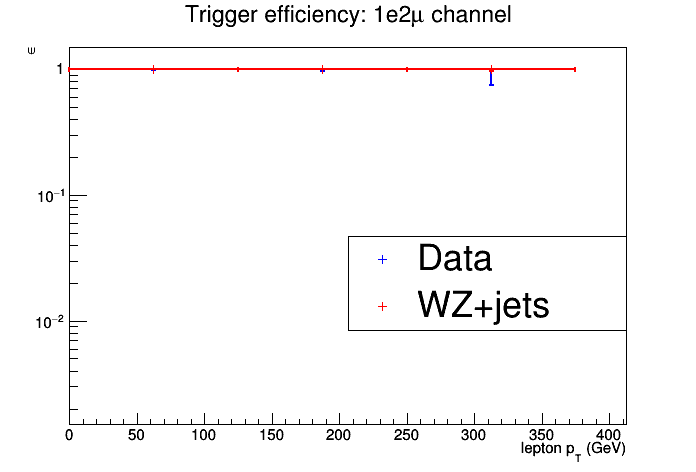
\includegraphics[width=0.48\textwidth]{Appendix/Figures/trigger/Triggereff/1e2mu/triggeff_1e2muhistPt.png}
		\label{image:triggeff_1e2muhistPt.png}
	}
	[In function of 2nd leading lepton in \pt]{
		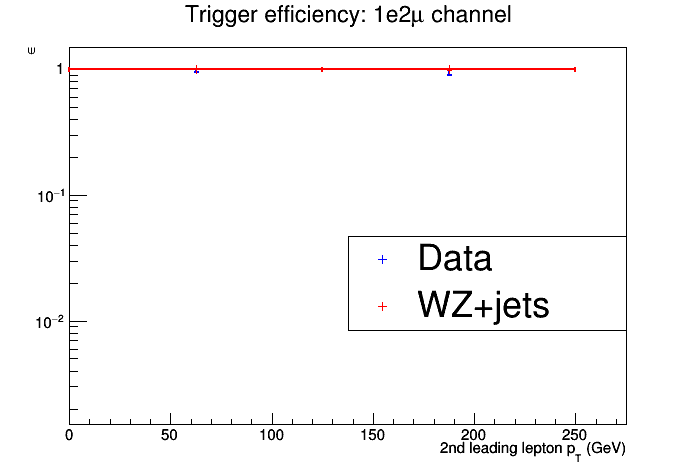
\includegraphics[width=0.48\textwidth]{Appendix/Figures/trigger/Triggereff/1e2mu/triggeff_1e2muhistPt_2ndleadinglep.png}
		\label{image:triggeff_1e2muhistPt_2ndleadinglep.png}
	}
	\newline
	[In function of 3d leading lepton in \pt]{
		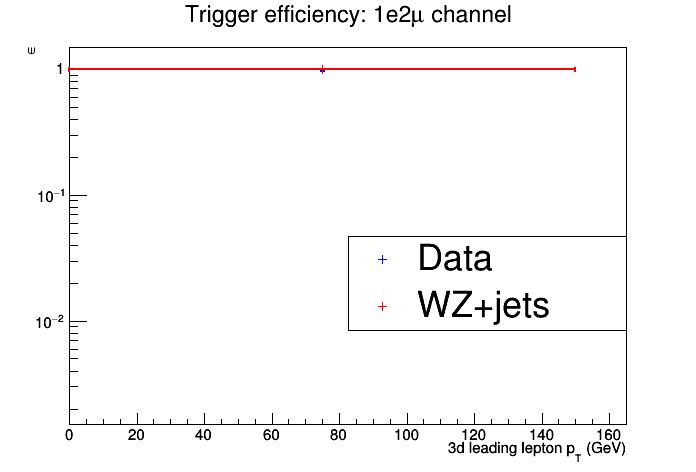
\includegraphics[width=0.48\textwidth]{Appendix/Figures/trigger/Triggereff/1e2mu/triggeff_1e2muhistPt_3dleadinglep.png}
		\label{image:triggeff_1e2muhistPt_3dleadinglep.png}
	}
	[In function of leading lepton in \pt]{
		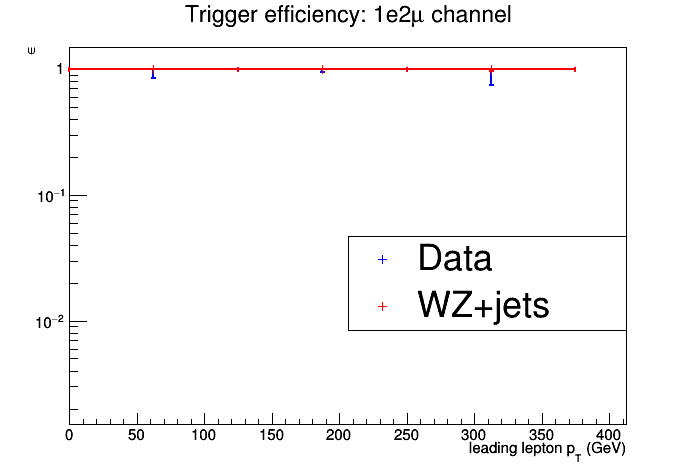
\includegraphics[width=0.48\textwidth]{Appendix/Figures/trigger/Triggereff/1e2mu/triggeff_1e2muhistPt_leadinglep.png}
		\label{image:triggeff_1e2muhistPt_leadinglep.png}
	}
	\caption{The trigger efficiencies measured as a function of lepton \pt, using the dataset collected by \Etmis\ triggers and \WZ\ simulation, after a 3 lepton and jets selection, in the Z mass window. All corrections to simulation are applied. 1e2$\mu$ channel.}
	\label{image:FigurestriggerTriggereff1e2mu}
\end{figure}

\begin{figure}[tb]
	[In function of lepton \pt]{
		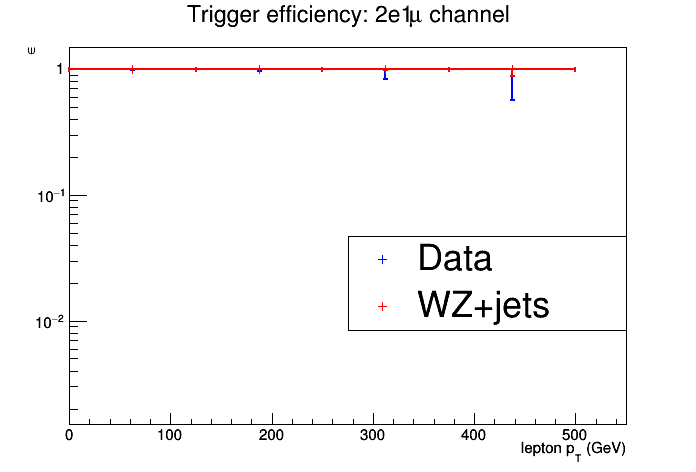
\includegraphics[width=0.48\textwidth]{Appendix/Figures/trigger/Triggereff/2e1mu/triggeff_2e1muhistPt.png}
		\label{image:triggeff_2e1muhistPt.png}
	}
	[In function of 2nd leading lepton in \pt]{
		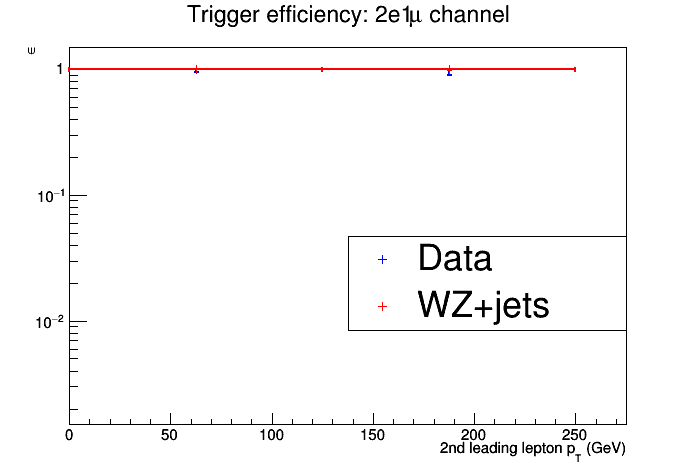
\includegraphics[width=0.48\textwidth]{Appendix/Figures/trigger/Triggereff/2e1mu/triggeff_2e1muhistPt_2ndleadinglep.png}
		\label{image:triggeff_2e1muhistPt_2ndleadinglep.png}
	}
	\newline
	[In function of 3d leading lepton in \pt]{
		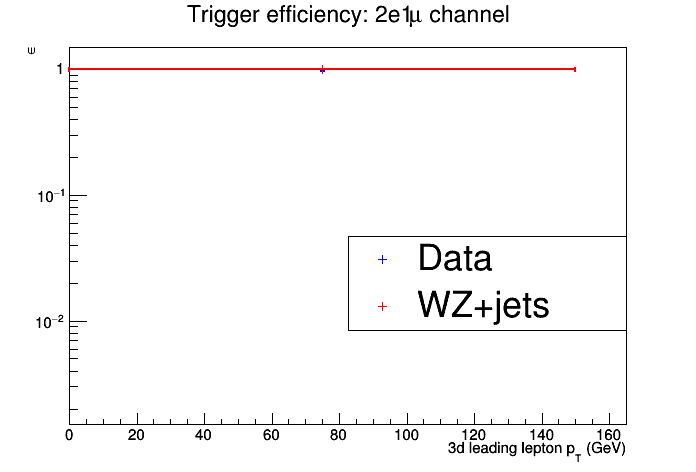
\includegraphics[width=0.48\textwidth]{Appendix/Figures/trigger/Triggereff/2e1mu/triggeff_2e1muhistPt_3dleadinglep.png}
		\label{image:triggeff_2e1muhistPt_3dleadinglep.png}
	}
	[In function of leading lepton in \pt]{
		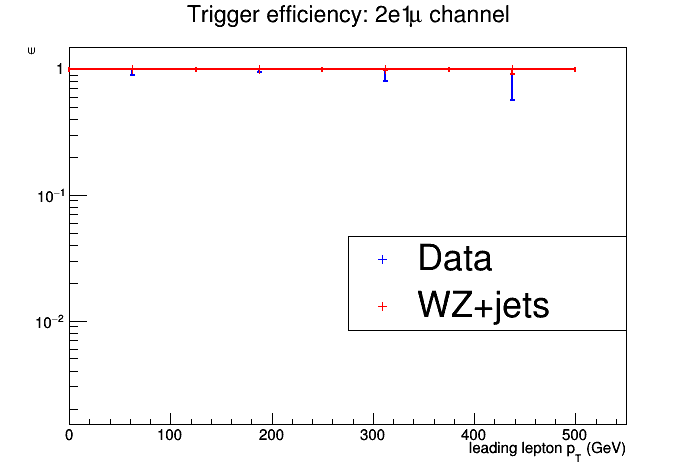
\includegraphics[width=0.48\textwidth]{Appendix/Figures/trigger/Triggereff/2e1mu/triggeff_2e1muhistPt_leadinglep.png}
		\label{image:triggeff_2e1muhistPt_leadinglep.png}
	}
	\caption{The trigger efficiencies measured as a function of lepton \pt, using the dataset collected by \Etmis\ triggers and \WZ\ simulation, after a 3 lepton and jets selection, in the Z mass window. All corrections to simulation are applied. 2e1$\mu$ channel.}
	\label{image:FigurestriggerTriggereff2e1mu}
\end{figure}

\begin{figure}[tb]
	[In function of lepton \pt]{
		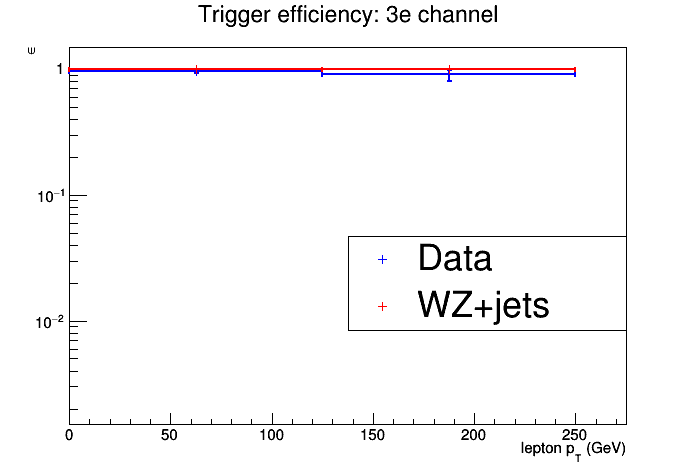
\includegraphics[width=0.48\textwidth]{Appendix/Figures/trigger/Triggereff/3e/triggeff_3ehistPt.png}
		\label{image:triggeff_3ehistPt.png}
	}
	[In function of 2nd leading lepton in \pt]{
		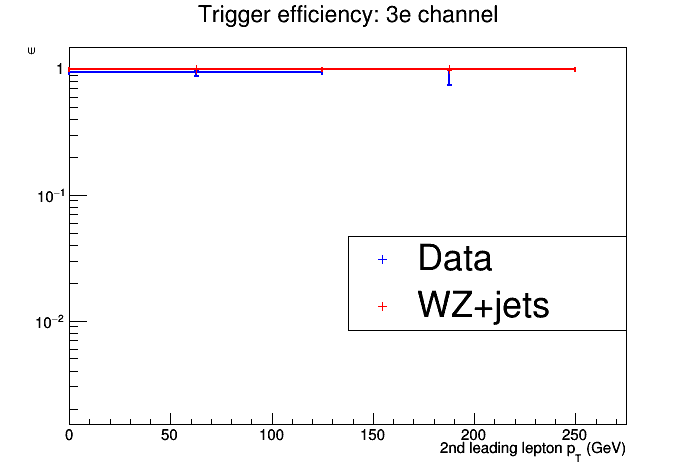
\includegraphics[width=0.48\textwidth]{Appendix/Figures/trigger/Triggereff/3e/triggeff_3ehistPt_2ndleadinglep.png}
		\label{image:triggeff_3ehistPt_2ndleadinglep.png}
	}
	\newline
	[In function of 3d leading lepton in \pt]{
		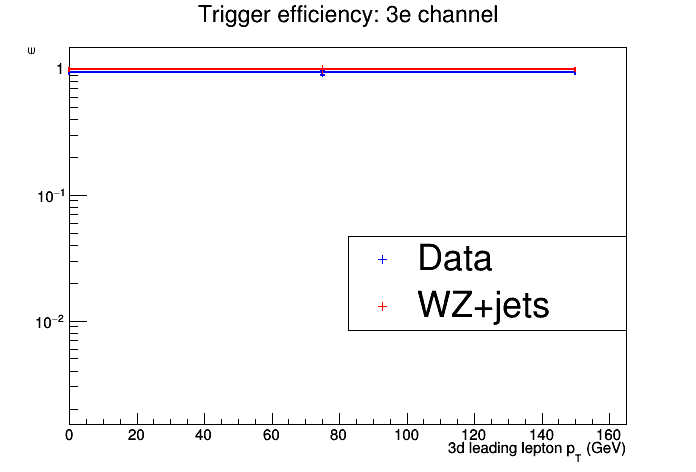
\includegraphics[width=0.48\textwidth]{Appendix/Figures/trigger/Triggereff/3e/triggeff_3ehistPt_3dleadinglep.png}
		\label{image:triggeff_3ehistPt_3dleadinglep.png}
	}
	[In function of leading lepton in \pt]{
		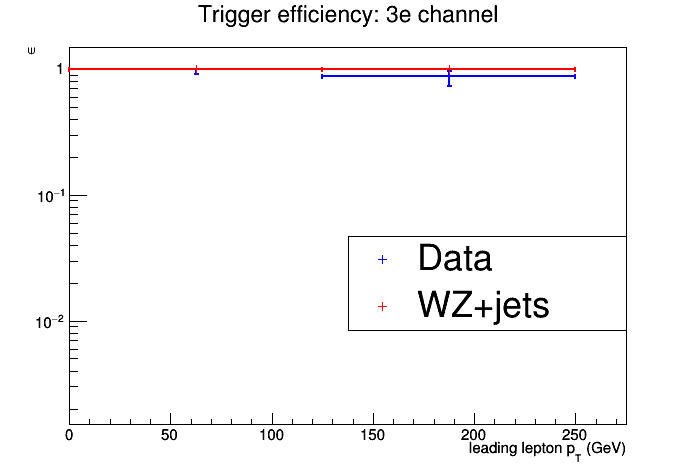
\includegraphics[width=0.48\textwidth]{Appendix/Figures/trigger/Triggereff/3e/triggeff_3ehistPt_leadinglep.png}
		\label{image:triggeff_3ehistPt_leadinglep.png}
	}
	\caption{The trigger efficiencies measured as a function of lepton \pt, using the dataset collected by \Etmis\ triggers and \WZ\ simulation, after a 3 lepton and jets selection, in the Z mass window. All corrections to simulation are applied. 3e channel.}
	\label{image:FigurestriggerTriggereff3e}
\end{figure}

\begin{figure}[tb]
	[In function of lepton \pt]{
		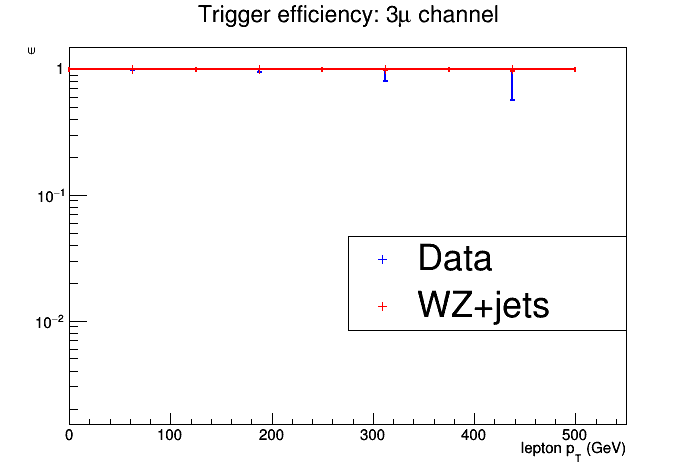
\includegraphics[width=0.48\textwidth]{Appendix/Figures/trigger/Triggereff/3mu/triggeff_3muhistPt.png}
		\label{image:triggeff_3muhistPt.png}
	}
	[In function of 2nd leading lepton in \pt]{
		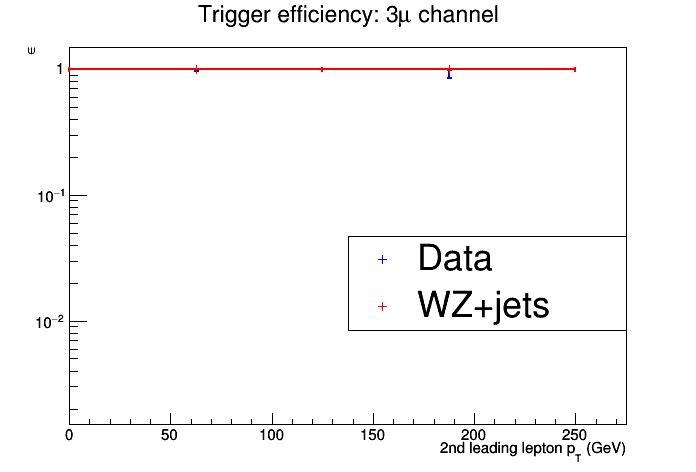
\includegraphics[width=0.48\textwidth]{Appendix/Figures/trigger/Triggereff/3mu/triggeff_3muhistPt_2ndleadinglep.png}
		\label{image:triggeff_3muhistPt_2ndleadinglep.png}
	}
	\newline
	[In function of 3d leading lepton in \pt]{
		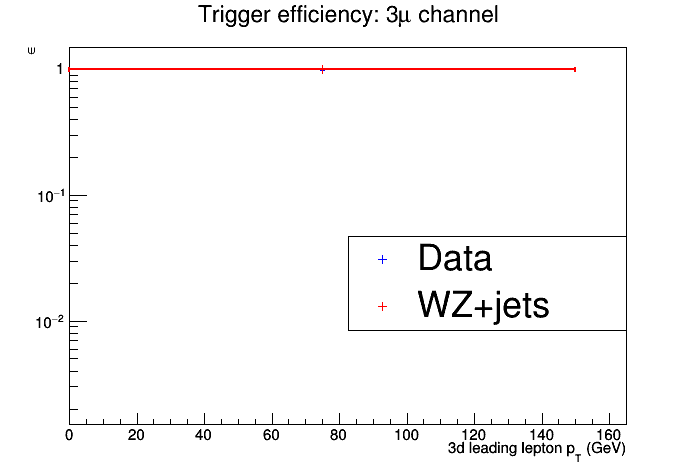
\includegraphics[width=0.48\textwidth]{Appendix/Figures/trigger/Triggereff/3mu/triggeff_3muhistPt_3dleadinglep.png}
		\label{image:triggeff_3muhistPt_3dleadinglep.png}
	}
	[In function of leading lepton in \pt]{
		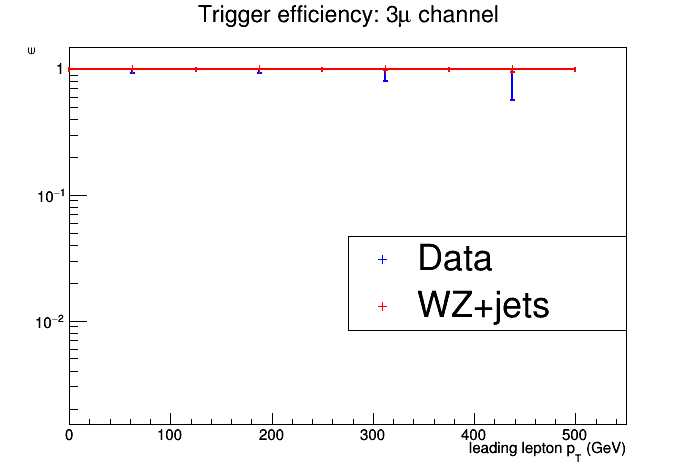
\includegraphics[width=0.48\textwidth]{Appendix/Figures/trigger/Triggereff/3mu/triggeff_3muhistPt_leadinglep.png}
		\label{image:triggeff_3muhistPt_leadinglep.png}
	}
	\caption{The trigger efficiencies measured as a function of lepton \pt, using the dataset collected by \Etmis\ triggers and \WZ\ simulation, after a 3 lepton and jets selection, in the Z mass window. All corrections to simulation are applied. 3$\mu$ channel.}
	\label{image:FigurestriggerTriggereff3mu}
\end{figure}

\begin{figure}[tb]
	[In function of lepton \pt]{
		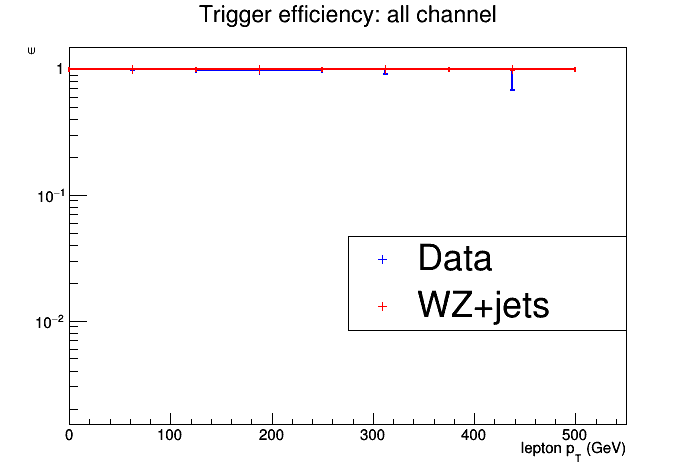
\includegraphics[width=0.48\textwidth]{Appendix/Figures/trigger/Triggereff/all/triggeff_allhistPt.png}
		\label{image:triggeff_allhistPt.png}
	}
	[In function of 2nd leading lepton in \pt]{
		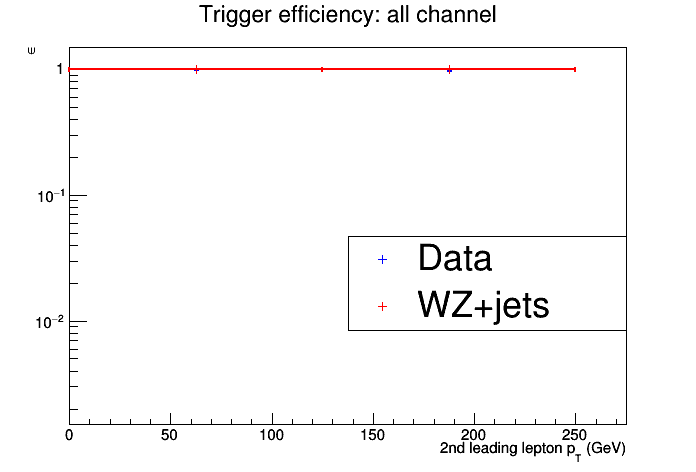
\includegraphics[width=0.48\textwidth]{Appendix/Figures/trigger/Triggereff/all/triggeff_allhistPt_2ndleadinglep.png}
		\label{image:triggeff_allhistPt_2ndleadinglep.png}
	}
	\newline
	[In function of 3d leading lepton in \pt]{
		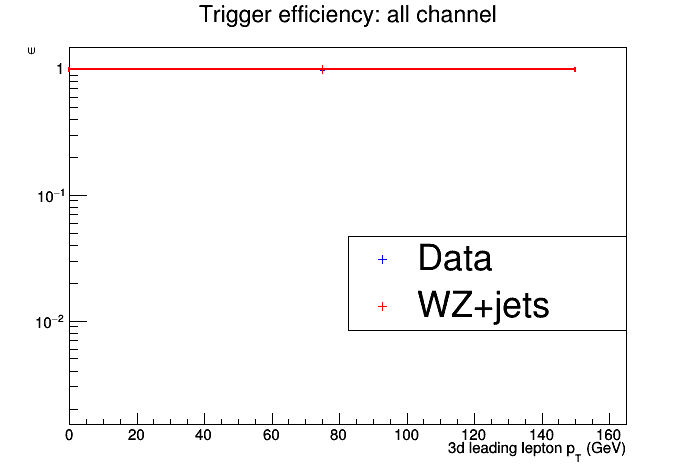
\includegraphics[width=0.48\textwidth]{Appendix/Figures/trigger/Triggereff/all/triggeff_allhistPt_3dleadinglep.png}
		\label{image:triggeff_allhistPt_3dleadinglep.png}
	}
	[In function of leading lepton in \pt]{
		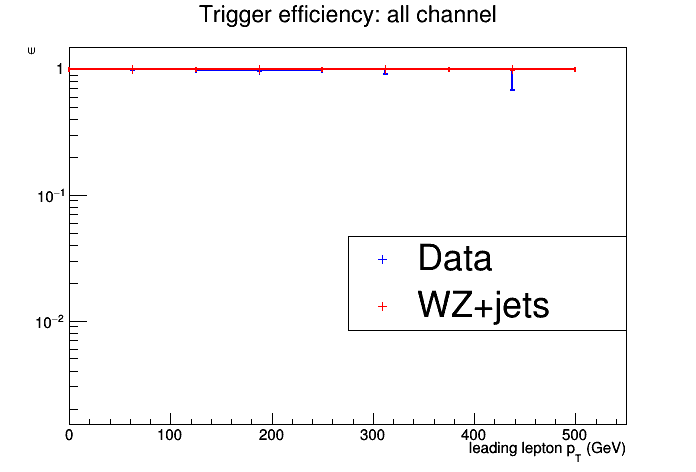
\includegraphics[width=0.48\textwidth]{Appendix/Figures/trigger/Triggereff/all/triggeff_allhistPt_leadinglep.png}
		\label{image:triggeff_allhistPt_leadinglep.png}
	}
	\caption{The trigger efficiencies measured as a function of lepton \pt, using the dataset collected by \Etmis\ triggers and \WZ\ simulation, after a 3 lepton and jets selection, in the Z mass window. All corrections to simulation are applied. All channel.}
	\label{image:FigurestriggerTriggereffall}
\end{figure}

\begin{figure}[tb]
	[In function of lepton \pt]{
		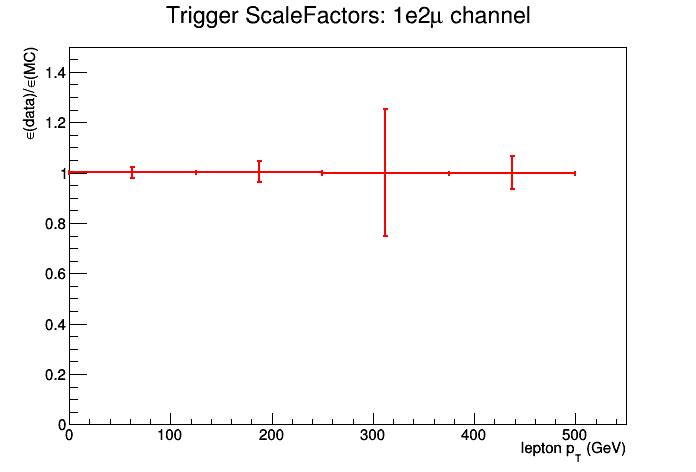
\includegraphics[width=0.48\textwidth]{Appendix/Figures/trigger/ScaleFactors/1e2mu/SF_trigger_1e2muhistPt.png}
		\label{image:1e2muhistPt.png}
	}
	[In function of 2nd leading lepton in \pt]{
		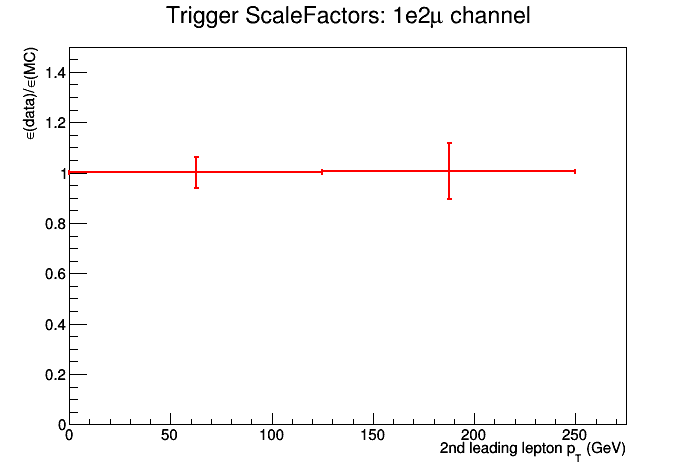
\includegraphics[width=0.48\textwidth]{Appendix/Figures/trigger/ScaleFactors/1e2mu/SF_trigger_1e2muhistPt_2ndleadinglep.png}
		\label{image:1e2muhistPt_2ndleadinglep.png}
	}
	\newline
	[In function of 3d leading lepton in \pt]{
		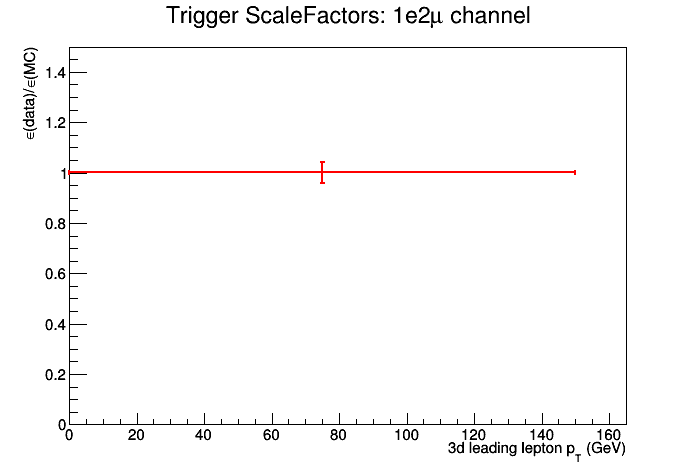
\includegraphics[width=0.48\textwidth]{Appendix/Figures/trigger/ScaleFactors/1e2mu/SF_trigger_1e2muhistPt_3dleadinglep.png}
		\label{image:1e2muhistPt_3dleadinglep.png}
	}
	[In function of leading lepton in \pt]{
		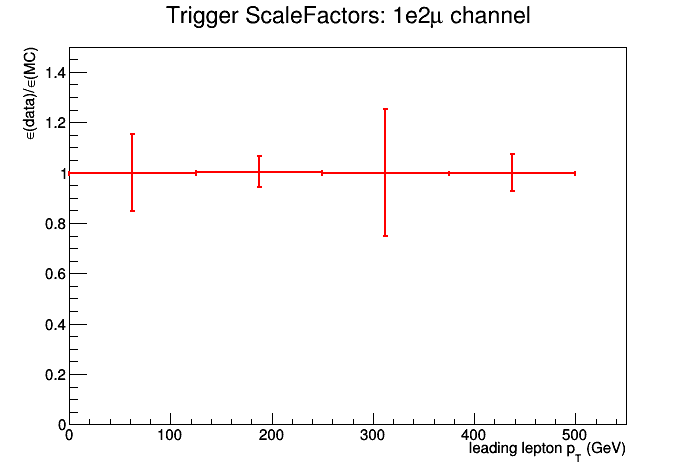
\includegraphics[width=0.48\textwidth]{Appendix/Figures/trigger/ScaleFactors/1e2mu/SF_trigger_1e2muhistPt_leadinglep.png}
		\label{image:1e2muhistPt_leadinglep.png}
	}
	\caption{The trigger scale factors measured as a function of lepton \pt, using the dataset collected by \Etmis\ triggers and \WZ\ simulation, after a 3 lepton and jets selection, in the Z mass window. All corrections to simulation are applied. 1e2$\mu$ channel.}
	\label{image:FigurestriggerScaleFactors1e2mu}
\end{figure}

\begin{figure}[tb]
	[In function of lepton \pt]{
		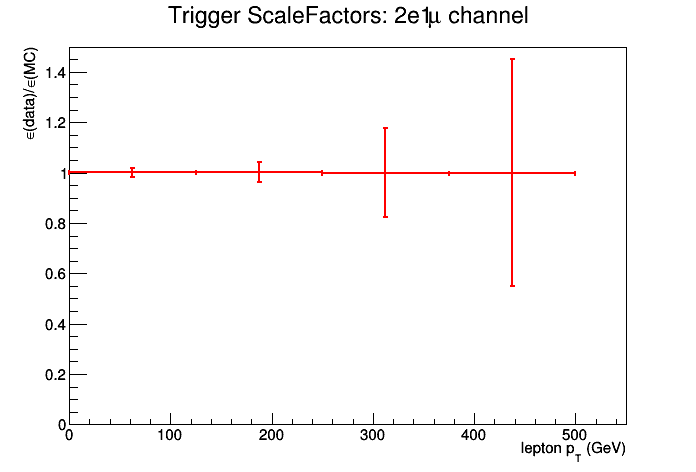
\includegraphics[width=0.48\textwidth]{Appendix/Figures/trigger/ScaleFactors/2e1mu/SF_trigger_2e1muhistPt.png}
		\label{image:2e1muhistPt.png}
	}
	[In function of 2nd leading lepton in \pt]{
		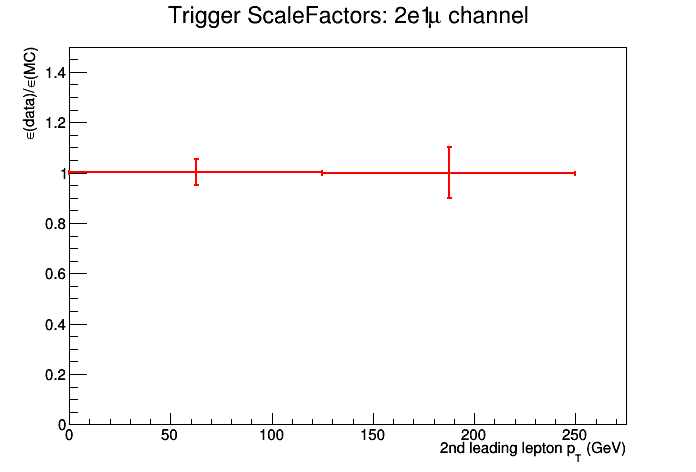
\includegraphics[width=0.48\textwidth]{Appendix/Figures/trigger/ScaleFactors/2e1mu/SF_trigger_2e1muhistPt_2ndleadinglep.png}
		\label{image:2e1muhistPt_2ndleadinglep.png}
	}
	\newline
	[In function of 3d leading lepton in \pt]{
		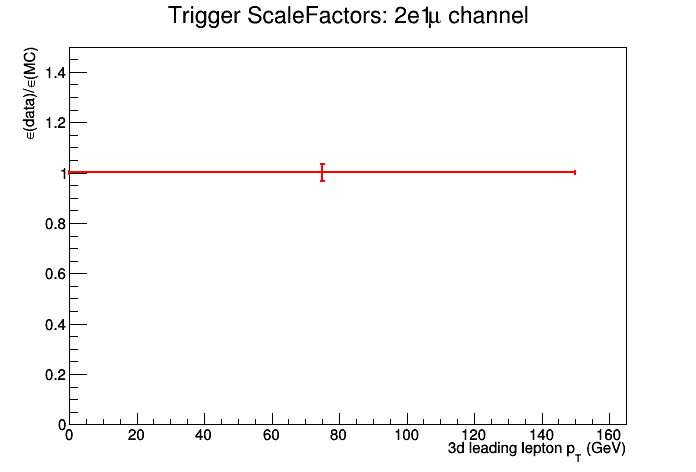
\includegraphics[width=0.48\textwidth]{Appendix/Figures/trigger/ScaleFactors/2e1mu/SF_trigger_2e1muhistPt_3dleadinglep.png}
		\label{image:2e1muhistPt_3dleadinglep.png}
	}
	[In function of leading lepton in \pt]{
		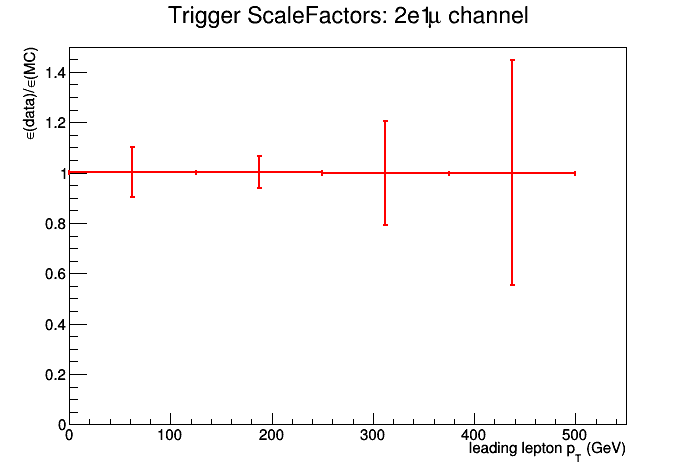
\includegraphics[width=0.48\textwidth]{Appendix/Figures/trigger/ScaleFactors/2e1mu/SF_trigger_2e1muhistPt_leadinglep.png}
		\label{image:2e1muhistPt_leadinglep.png}
	}
	\caption{The trigger scale factors measured as a function of lepton \pt, using the dataset collected by \Etmis\ triggers and \WZ\ simulation, after a 3 lepton and jets selection, in the Z mass window. All corrections to simulation are applied. 2e1$\mu$ channel.}
	\label{image:FigurestriggerScaleFactors2e1mu}
\end{figure}

\begin{figure}[tb]
	[In function of lepton \pt]{
		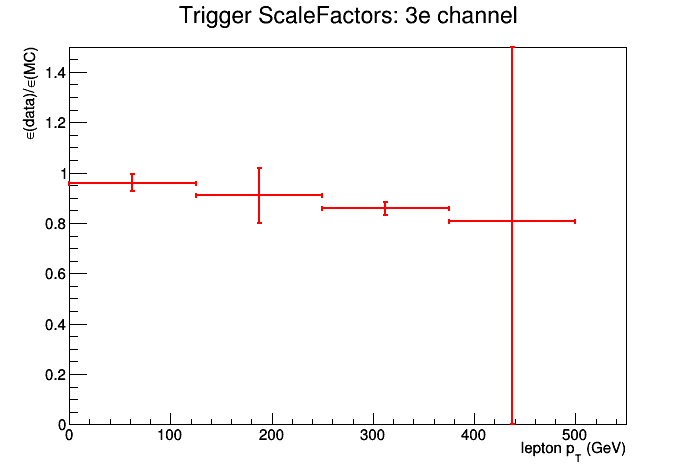
\includegraphics[width=0.48\textwidth]{Appendix/Figures/trigger/ScaleFactors/3e/SF_trigger_3ehistPt.png}
		\label{image:3ehistPt.png}
	}
	[In function of 2nd leading lepton in \pt]{
		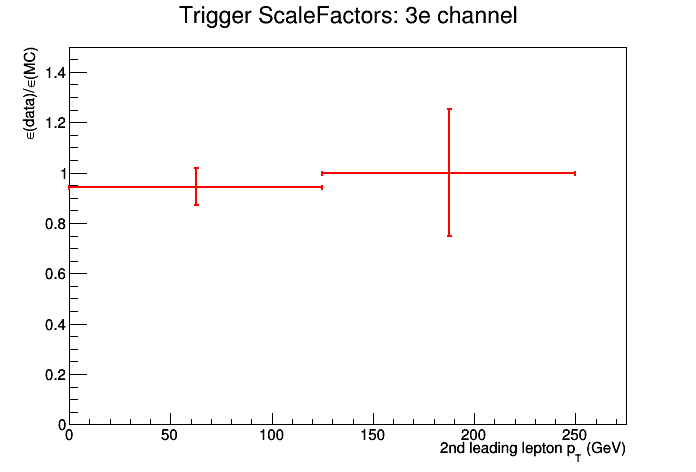
\includegraphics[width=0.48\textwidth]{Appendix/Figures/trigger/ScaleFactors/3e/SF_trigger_3ehistPt_2ndleadinglep.png}
		\label{image:3ehistPt_2ndleadinglep.png}
	}
	\newline
	[In function of 3d leading lepton in \pt]{
		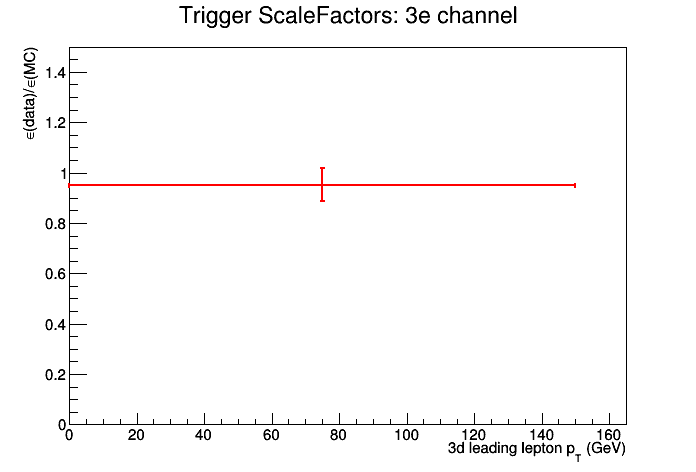
\includegraphics[width=0.48\textwidth]{Appendix/Figures/trigger/ScaleFactors/3e/SF_trigger_3ehistPt_3dleadinglep.png}
		\label{image:3ehistPt_3dleadinglep.png}
	}
	[In function of leading lepton in \pt]{
		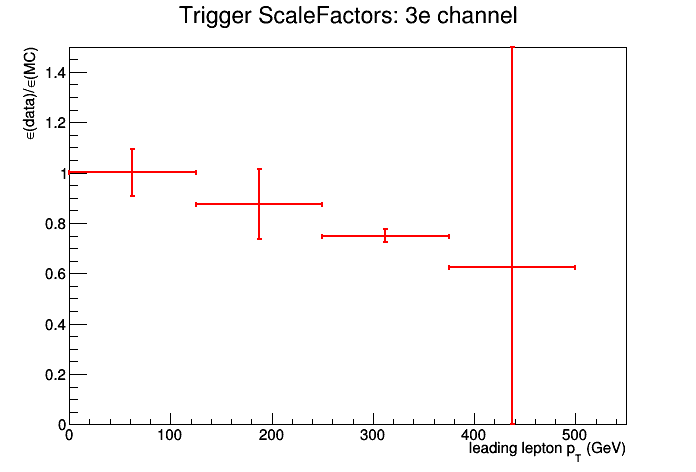
\includegraphics[width=0.48\textwidth]{Appendix/Figures/trigger/ScaleFactors/3e/SF_trigger_3ehistPt_leadinglep.png}
		\label{image:3ehistPt_leadinglep.png}
	}
	\caption{The trigger scale factors measured as a function of lepton \pt, using the dataset collected by \Etmis\ triggers and \WZ\ simulation, after a 3 lepton and jets selection, in the Z mass window. All corrections to simulation are applied. 3e channel.}
	\label{image:FigurestriggerScaleFactors3e}
\end{figure}

\begin{figure}[tb]
	[In function of lepton \pt]{
		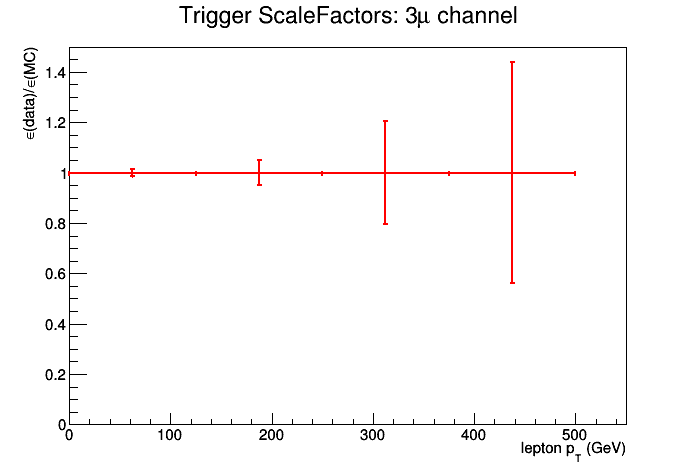
\includegraphics[width=0.48\textwidth]{Appendix/Figures/trigger/ScaleFactors/3mu/SF_trigger_3muhistPt.png}
		\label{image:3muhistPt.png}
	}
	[In function of 2nd leading lepton in \pt]{
		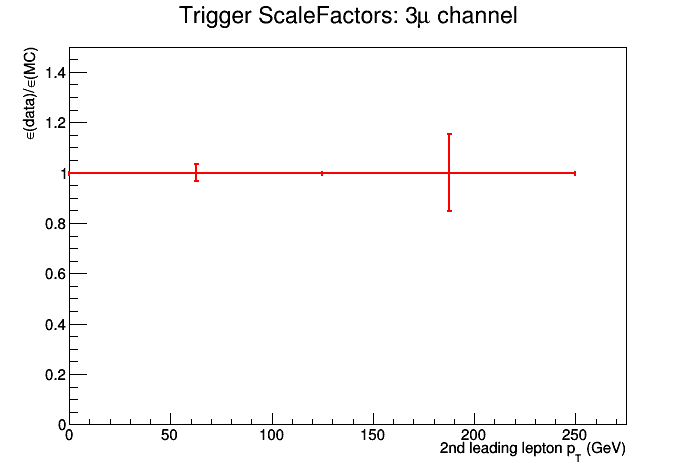
\includegraphics[width=0.48\textwidth]{Appendix/Figures/trigger/ScaleFactors/3mu/SF_trigger_3muhistPt_2ndleadinglep.png}
		\label{image:3muhistPt_2ndleadinglep.png}
	}
	\newline
	[In function of 3d leading lepton in \pt]{
		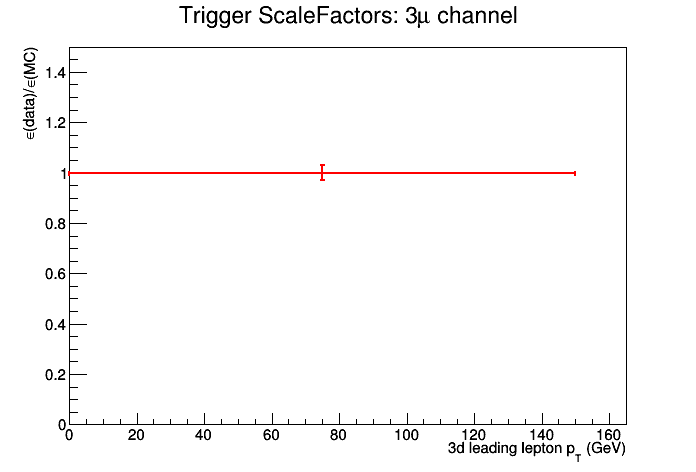
\includegraphics[width=0.48\textwidth]{Appendix/Figures/trigger/ScaleFactors/3mu/SF_trigger_3muhistPt_3dleadinglep.png}
		\label{image:3muhistPt_3dleadinglep.png}
	}
	[In function of leading lepton in \pt]{
		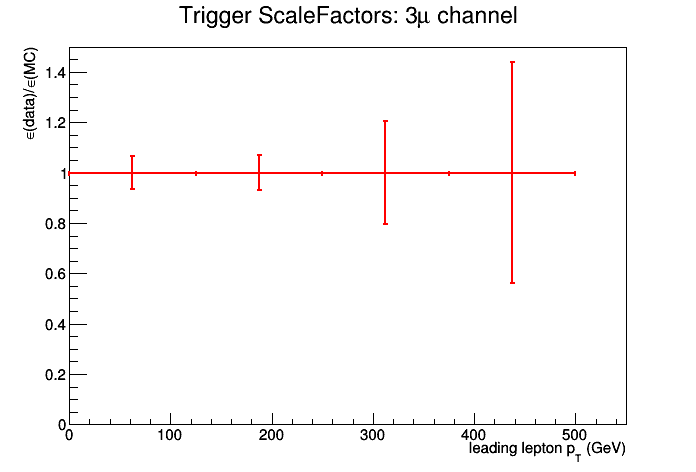
\includegraphics[width=0.48\textwidth]{Appendix/Figures/trigger/ScaleFactors/3mu/SF_trigger_3muhistPt_leadinglep.png}
		\label{image:3muhistPt_leadinglep.png}
	}
	\caption{The trigger scale factors measured as a function of lepton \pt, using the dataset collected by \Etmis\ triggers and \WZ\ simulation, after a 3 lepton and jets selection, in the Z mass window. All corrections to simulation are applied. 3$\mu$ channel.}
	\label{image:FigurestriggerScaleFactors3mu}
\end{figure}

\begin{figure}[tb]
	[In function of lepton \pt]{
		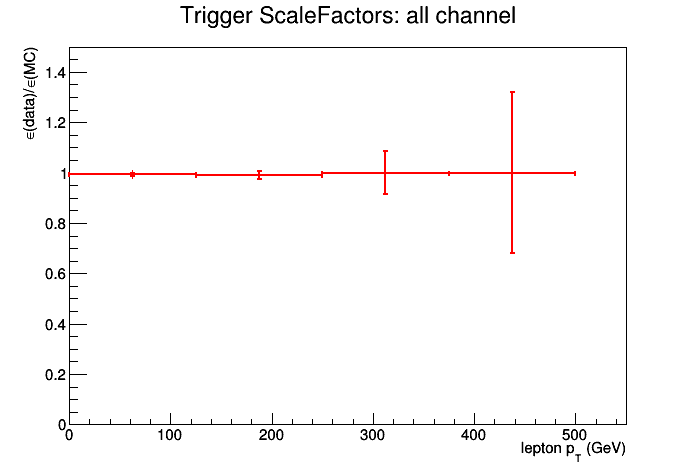
\includegraphics[width=0.48\textwidth]{Appendix/Figures/trigger/ScaleFactors/all/SF_trigger_allhistPt.png}
		\label{image:allhistPt.png}
	}
	[In function of 2nd leading lepton in \pt]{
		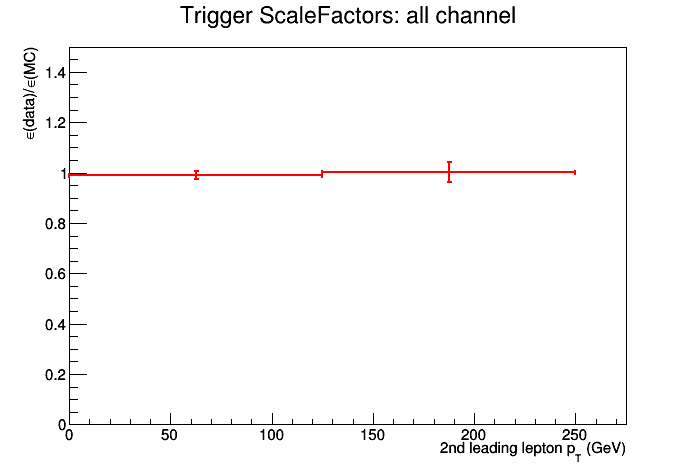
\includegraphics[width=0.48\textwidth]{Appendix/Figures/trigger/ScaleFactors/all/SF_trigger_allhistPt_2ndleadinglep.png}
		\label{image:allhistPt_2ndleadinglep.png}
	}
	\newline
	[In function of 3d leading lepton in \pt]{
		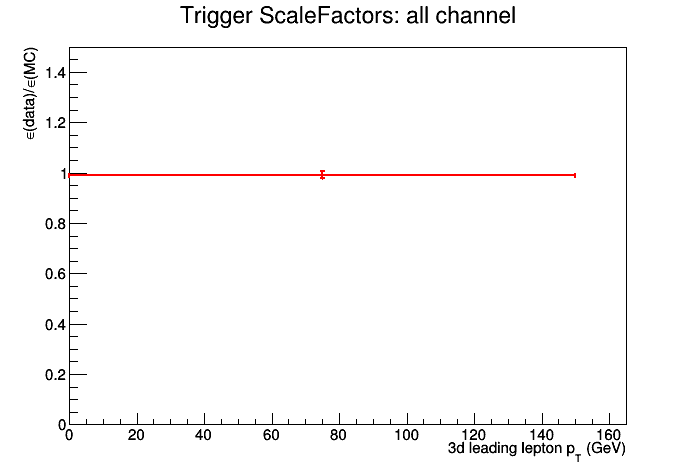
\includegraphics[width=0.48\textwidth]{Appendix/Figures/trigger/ScaleFactors/all/SF_trigger_allhistPt_3dleadinglep.png}
		\label{image:allhistPt_3dleadinglep.png}
	}
	[In function of leading lepton in \pt]{
		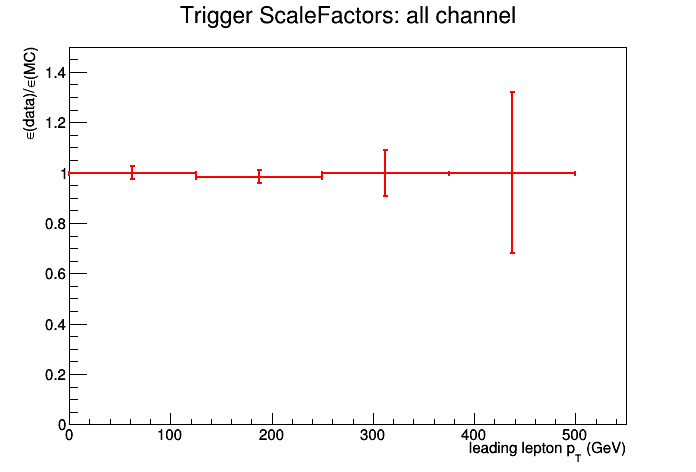
\includegraphics[width=0.48\textwidth]{Appendix/Figures/trigger/ScaleFactors/all/SF_trigger_allhistPt_leadinglep.png}
		\label{image:allhistPt_leadinglep.png}
	}
	\caption{The trigger scale factors measured as a function of lepton \pt, using the dataset collected by \Etmis\ triggers and \WZ\ simulation, after a 3 lepton and jets selection, in the Z mass window. All corrections to simulation are applied. All channel.}
	\label{image:FigurestriggerScaleFactorsall}
\end{figure}


\chapter{Dilepton controlplots}
\label{app:controldilep}


\chapter{Statistical independent regions}
\label{app:tablestr}